\begin{figure}[t]
\centering
\begin{tabular}{c c c}
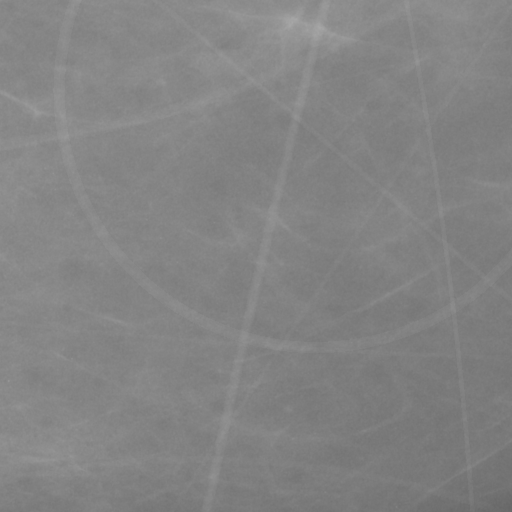
\includegraphics[width=0.3\columnwidth]{\figpath/mammo/synth_lines} &
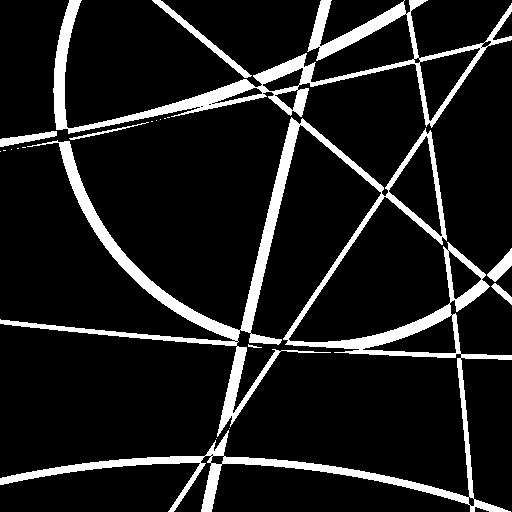
\includegraphics[width=0.3\columnwidth]{\figpath/mammo/synth_mask} &
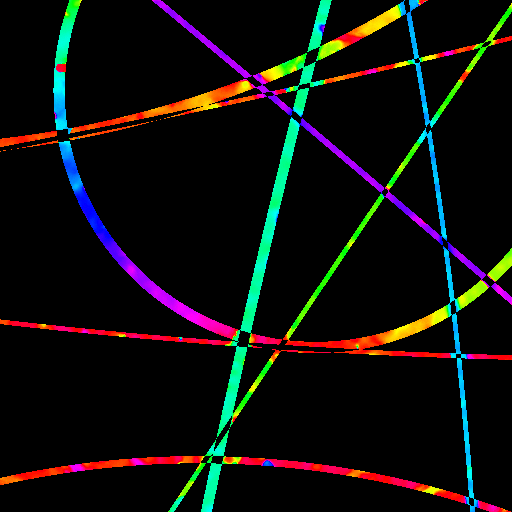
\includegraphics[width=0.3\columnwidth]{\figpath/mammo/synth_result} \\
(a) & (b) & (c)
\end{tabular}
%
\caption{Synthetic mammographic images: %
(a) input image; %
(b) mask indicating pixels belonging to a vessel; %
(c) orientation (indicated by colour) estimated using Random Forest regression over \dtcwt{} features. The mask was not used to estimate orientation.%
}
\label{f:synth_mammography}
\end{figure}
